
% !TeX spellcheck = de_DE

\documentclass{article}

\usepackage[ngerman]{babel}
\usepackage{graphicx}
\usepackage{indentfirst}
\usepackage{hyperref}
\usepackage{geometry}
\usepackage{changepage}
\usepackage{booktabs}
\usepackage{float}
\usepackage{tabulary}
\usepackage{xcolor}
\usepackage{multirow}
\usepackage{caption}
\usepackage{subcaption}
\usepackage{lscape}
\usepackage{colortbl}
\usepackage{listings}

\graphicspath{ {./images/} }
\setlength\parindent{0pt}

\hypersetup{
    colorlinks,
    linkcolor={cyan!50!black},
    citecolor={blue!50!black},
    urlcolor={blue!80!black}
}

\makeatletter
\newcommand{\sectionauthor}[1]{
	{\parindent 0em \large \scshape Autor: #1 \par \nobreak \vspace*{1em}}
	\@afterheading
}
\newcommand{\specification}[3]{
	{\parindent 0.5em \hangindent 3em \hypertarget{spec:#1:#2}{\textbf{/#1#2/}} #3 \par \nobreak \vspace*{0.5em}}
}
\makeatother

\title{Bibliotheksanwendung - Feinspezifikation}
\date{\today\\v1.1}
\author{
	Ivan Charviakou\\
	León Liehr\\
	Mohamad Najjar\\
	Jonas Picker\\
	Sergei Pravdin
}

\begin{document}
\maketitle
\begin{figure}[H]
	\centering
	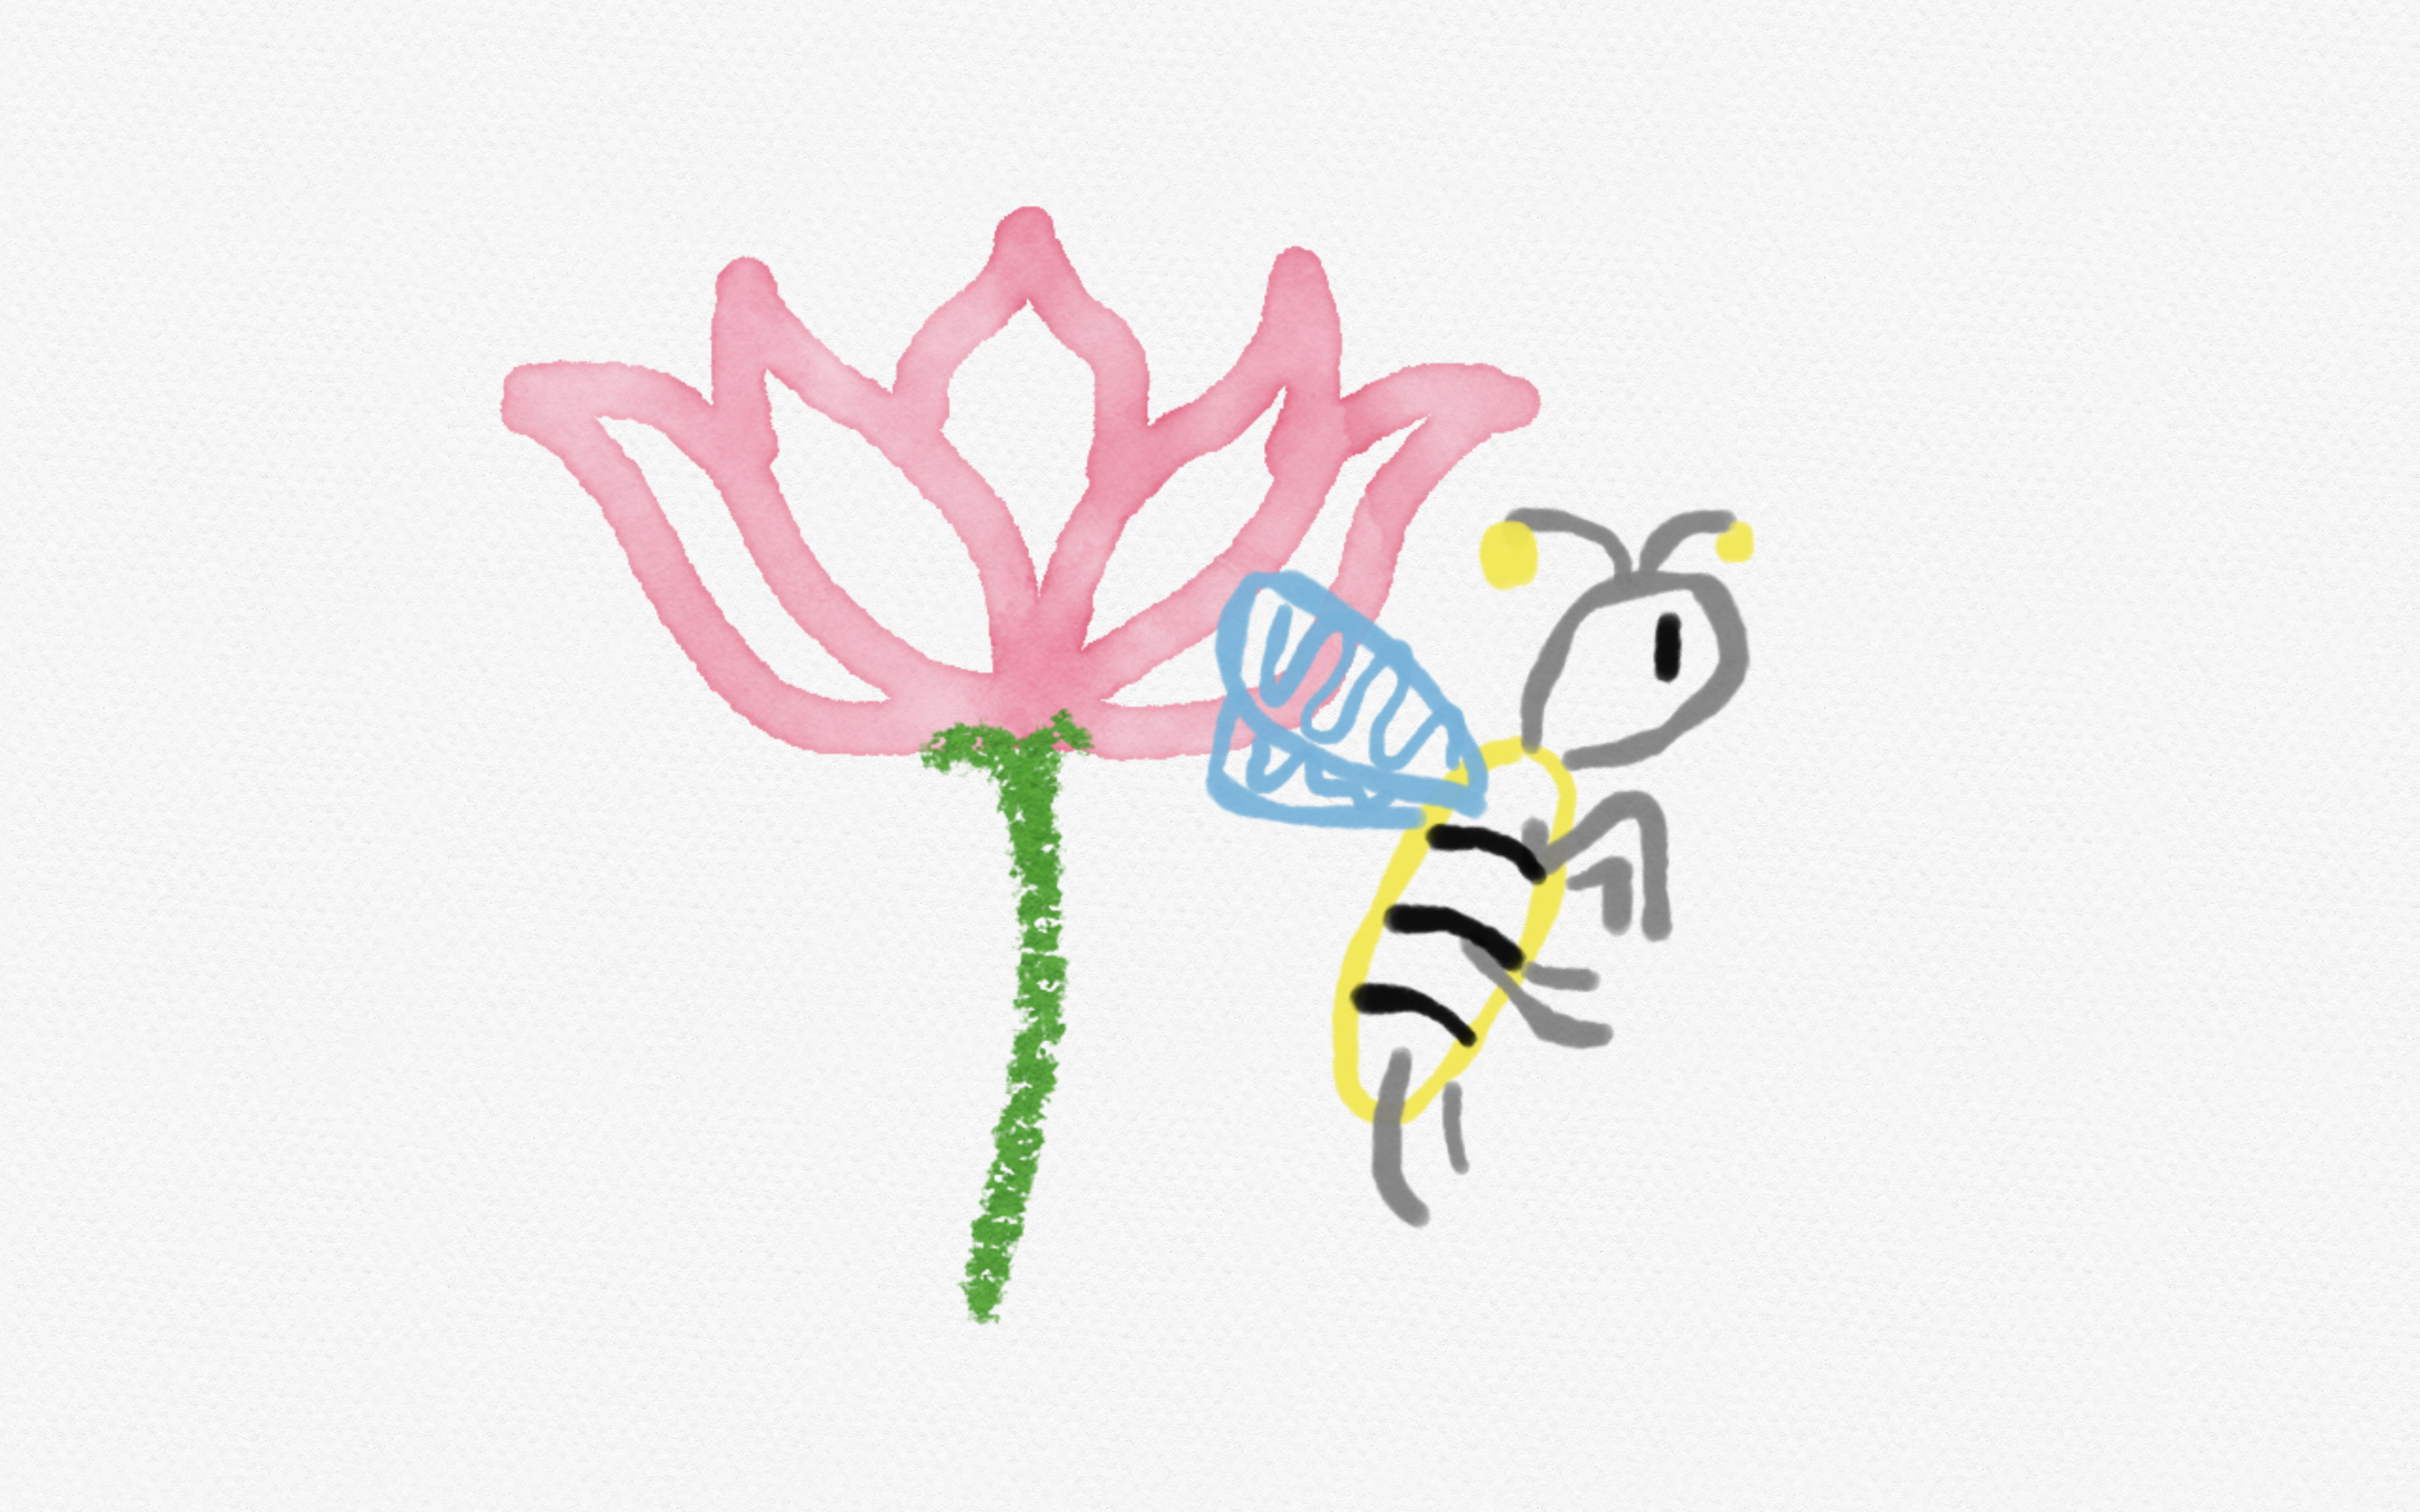
\includegraphics[width = 30em]{Logo}
\end{figure}
\newpage
\tableofcontents
\newpage

%----------------------------------------------------------------------Kapitel 1--------------------------------------------------------------------------------------------

\section{Meilensteine}
\sectionauthor{Jonas Picker}
Die Implementierungsphase wird drei Wochen dauern und in 3 gleiche Zeitabschnitte unterteilt, in denen wesentliche Funktionalitäten fertiggestellt werden sollen. Allgemein liegt der Schwerpunkt auf einer vertikale, testbare Realisierung einzelner Funktionen, jedoch müssen gewisse Kernmodule direkt im ersten Milestone abgearbeitet werden. 
\subsection{Meilenstein 1}
\textbf{Fertigstellungsdatum:} 
\subsection{Meilenstein 2}
\textbf{Fertigstellungsdatum:} 
\subsection{Meilenstein 3}
\textbf{Fertigstellungsdatum:} 
%----------------------------------------------------------------------Kapitel 2--------------------------------------------------------------------------------------------

\section{Arbeitspakete}

%----------------------------------------------------------------------Kapitel 3--------------------------------------------------------------------------------------------

\section{PERT-Diagramm}

%----------------------------------------------------------------------Kapitel 4--------------------------------------------------------------------------------------------

\section{Spezialgebiete}
\sectionauthor{Jonas Picker}
Die Vielzahl der verwendeten Technologien erfordert eine Spezialisierung der einzelnen Teammitglieder. Spezialgebiete werden unten aufgelistet.
\begin{table}[H]
\centering
\begin{tabular}{| p{6cm} | p{6cm} |}
	\hline
     	git & León Liehr \\
     	\hline
     	JSF Internationalisierung & León Liehr \\
     	\hline
    	JSF Templates & León Liehr \\	
     	\hline
     	JSF Components & León Liehr \\
     	\hline
     	\hline
     	LaTeX & Ivan Charviakou \\
     	\hline
     	RegEx & Ivan Charviakou \\
     	\hline
     	Jakarta Mail & Ivan Charviakou \\
     	\hline
     	JSF Validators & Ivan Charviakou \\
     	\hline
     	\hline
     	JSF Converters & Mohamad Najjar \\
    	\hline
    	 RSA & Mohamad Najjar \\
    	\hline
    	 CSS/Bootstrap & Mohamad Najjar \\
     	\hline
     	Listenabstraktion & Mohamad Najjar \\
     	\hline
     	\hline
     	SQL & Jonas Picker \\
    	\hline
    	JSF File Upload & Jonas Picker \\
     	\hline
     	JSF/CDI Scopes & Jonas Picker \\
     	\hline
     	SSL/TLS & Jonas Picker \\
     	\hline
     	Systemkonfiguration & Jonas Picker \\
     	\hline
     	\hline
     	Selenium & Sergei Pravdin \\
     	\hline
     	Logging & Sergei Pravdin \\
     	\hline
     	JUnit & Sergei Pravdin \\
     	\hline
\end{tabular}
\end{table}

%----------------------------------------------------------------------Kapitel 5--------------------------------------------------------------------------------------------

\section{Whitebox-Tests}


\end{document}
